\documentclass[12pt,a4paper]{article}%
%Options -- Point size:  10pt (default), 11pt, 12pt
%        -- Paper size:  letterpaper (default), a4paper, a5paper, b5paper
%                        legalpaper, executivepaper
%        -- Orientation  (portrait is the default)
%                        landscape
%        -- Print size:  oneside (default), twoside
%        -- Quality      final(default), draft
%        -- Title page   notitlepage, titlepage(default)
%        -- Columns      onecolumn(default), twocolumn
%        -- Equation numbering (equation numbers on the right is the default)
%                        leqno
%        -- Displayed equations (centered is the default)
%                        fleqn (equations start at the same distance from the right side)
%        -- Open bibliography style (closed is the default)
%                        openbib
% For instance the command
%           \documentclass[a4paper,12pt,leqno]{article}
% ensures that the paper size is a4, the fonts are typeset at the size 12p
% and the equation numbers are on the left side
%====================Tabelas==============================================
\usepackage{multirow}
%=============================Símbolos Matemáticos=====================================================================
\usepackage{amsmath}
\usepackage{amsfonts}
\usepackage{amssymb}
%=======================================Figuras===========================================================
\usepackage{graphicx}
%\usepackage{wrapfig}
\usepackage{float}
\usepackage{tikz}
%=====================================Língua e acentos=============================================================
\usepackage[brazil]{babel}
\usepackage[utf8]{inputenc}
\usepackage[T1]{fontenc}
%========================================Espaçamento==========================================================
\usepackage[top=3cm, bottom=2cm, left=2cm, right=2cm]{geometry}
\usepackage{indentfirst}
%=======================================Lista de códigos===========================================================
\usepackage{listings}                   % para formatar código-fonte
\lstset{numbers=left, numberstyle=\tiny, stepnumber=1, numbersep=5pt, basicstyle=\scriptsize , frame=trbl}
%======================================Latexdraw============================================================
%\usepackage[usenames,dvipsnames]{pstricks}
%\usepackage{epsfig}
%\usepackage{pst-grad} % For gradients
%\usepackage{pst-plot} % For axes
%==================================================================================================
%-------------------------------------------

\begin{document}

\begin{titlepage}
\begin{center}
\begin{figure}[h]

\includegraphics[scale=0.76]{Imagens/topdotitulo.png}
\end{figure}
\rule{\columnwidth}{1.5mm}
\

\large David Maykon Krepsky Silva\\
\large Havena Louise Pavão

\vspace{4cm}
{\bf \Large Título do Experimento}
\vspace{3.5cm}

\begin{flushright}
Data de realização do experimento:\\
XX de abril de 2016\\
Série/Turma:\\
1000/1011\\
Prof. Me. Jaime Laelson Jacob 
\end{flushright}

\vspace{3.2cm}
\today

\rule{\columnwidth}{1.3mm}
\end{center}
\end{titlepage}

\section{Resumo}
Análise prática de circuitos Moduladores e Demoduladores FM.
\newpage

\newpage

\tableofcontents

\newpage
\section{Introdução}
Modulação em frequência, ou também conhecido como FM, é um tipo de modulação na qual a informação é transmitida através de uma portadora variando-se sua frequência instantânea. Este tipo de modulação é amplamente utilizado para transmissão de voz, rádiodifusão e em alguns sistemas de transmissão de vídeo. No caso de sistemas de rádiodifusão, a grande vantagem de se utilizar modulação FM é a vantagem em cancelar ruídos que ocorrem naturalmente. 

\begin{figure}[H]
\centering
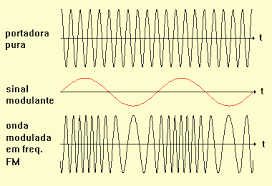
\includegraphics{imagem/sinal.png}
\caption{Relação entre Portadora, Sinal Modulante e Sinal FM.}
\label{fig:sinal}
\end{figure}

No entanto, uma desvantagem da modulação FM é de apresentar uma característica conhecido com efeito de captura, ou seja, se houverem dois ou mais sinais de FM em uma mesma frequência, o receptor irá captar o sinal de maior potência e ignorar os outros sinais de menores potência.


\newpage
\section{Teoria}

\subsection{Modulador FM com um transistor bipolar}
O circuito utilizado como transmissor do sinal de RF é caracterizado pelo uso de somente 1 transistor (circuito da figura \ref{fig:fm}).

\begin{figure}[H]
    \centering
    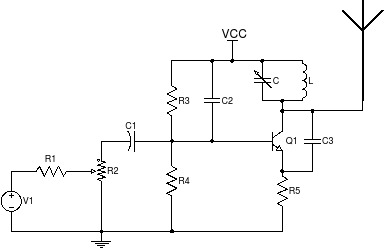
\includegraphics{imagem/fm.png}
    \caption{Transmissor FM a um transistor}
    \label{fig:fm}
\end{figure}

O seu funcionamento de dá da seguinte forma.
Primeiro, o sinal a ser transmitido, provindo da fonte V1, passa por um divisor resistivo de modo a controlar a potência de saída e também evitar a saturação do transistor Q1. Esse divisor resistivo é composto pelo resistor R1 e pelo potenciômetro R2, sendo o ajuste feito em R2.
Em seguida o sinal passa pelo capacitor de desacoplamento C1, o qual atua como um filtro passa-altas e tem o objetivo de remover a componente DC do sinal. O sinal então entra no modulador, que tem como elemento ativo Q1. Tal modulador consiste de um transistor na configuração emissor comum, responsável pela amplificação e misturamento do sinal com a portadora. A portadora é gerada através do circuito denominado \textit{tank}, composto por C e L, os quais operam filtrando o ruído térmico natural dos componentes na frequência $f_c$ e utilizam o transistor Q1 para amplificar a portadora, formando assim um circuito oscilador. O sinal modulado é encontrado então no coletor de Q1, onde se conecta a antena do sistema. A antena tem por trabalho irradiar o sinal modulado, gerando ondas eletro-magnéticas que viajarão através do espaço até o receptor.
O resistor R5 tem como função limitar a corrente que circula no transistor, evitando assim a queima do mesmo.


\begin{equation}
\label{equ:portadora}
f_c = \frac{1}{2 \pi \sqrt{LC}}
\end{equation}
 
A frequência da portadora é dada pela equação \ref{equ:portadora}, sendo possível ajustar a frequência de transmissão modificando o número de espiras do indutor ou através do uso de um capacitor variável.

O comprimento da antena também influencia na eficiência da transmissão, sendo recomendado uma antena com comprimento de:

\[
    d_{antena} = \frac{\lambda}{4}.
\]

Onde $\lambda$ é o comprimento de onda da portadora e é dado por:
\[
    \lambda = \frac{c}{f_c}.
\]
\newpage

Sendo $c$ a velocidade da luz.

\section{Metodologia e Desenvolvimento}
O experimento consistiu na montagem de um transmissor FM  modulação direta, conforme a Figura \ref{fig:transmissor}.
\begin{figure}[H]
\centering
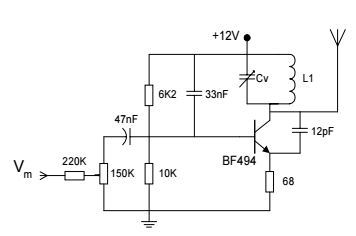
\includegraphics{imagem/transmissor.png}
\caption{Transmissor FM básico}
\label{fig:transmissor}
\end{figure}

A transmissão deveria ser feita na frequência de $88MHz$. No entanto, para isso foi necessário construir um Indutor $L_1$ que fizesse com que o circuito trabalhasse nesta frequência.
Como base para o enrolamento do indutor com núcleo de ar, optou-se por um tubo de caneta com diâmetro de $0,706cm$.
Tendo então uma área de $A=\pi \Bigg(\dfrac{0,706\times10^{-2}}{2}\Bigg)^2=39,147\times10^{-6}m^2$.

Para uma frequência de $88MHz$, tem-se
\begin{equation}
\begin{split}
\frac{1}{\sqrt{LC}}&=2\pi\cdot88\times10^6 \\L&=\frac{1}{C\cdot (2\pi\cdot88\times10^6)^2}\\
\end{split}
\end{equation}
Sendo $C=12pF$, o valor da indutância $L$ obtida foi $L=272,58nH$.

A indutância $L$ pode ser definida como
\begin{equation}
L=1,256\frac{A\cdot n^2 \times10^{-6}}{l}
\label{eq:1}
\end{equation}

Sendo $l$ o comprimento do indutor, $n$ o numero de espiras e $A$ a área do núcleo.

Como $l$ é definido por $l=n.d$, substituindo na Equação \ref{eq:1}, temos então que
\begin{equation}
L=1,256\frac{A\cdot n\times10^{-6}}{d}
\end{equation}

O fio utilizado foi um AWG19 com $0,912mm$ de diâmetro. Tendo então a área do núcleo, a indutância e o diâmetro do fio, tornou-se possível calcular o número de espiras do indutor.
\begin{equation}
n=\frac{L}{1,256}\frac{d}{A\times10^{-6}}=\frac{272,58[nH]}{1,256[\dfrac{H/m}{espiras}]}\frac{0,912[mm]}{39,147\times10^{-12}[m^2]}=5 \text{ espiras}
\end{equation}

Então para a montagem do transmissor FM na frequência de $88MHz$ utilizou-se de um indutor com 5 espiras de enrolamento.

Para construção da antena, optou-se por uma antena com um quarto do tamanho de comprimento de onda.
\begin{equation}
\frac{\lambda}{4}=\frac{c}{4f}=\frac{3\times10^8}{4\cdot 88\times10^6}=0,85m
\end{equation}

Como sinal modulante, foi utilizado um gerador de onda senoidal na frequência de $1kHz$ com $2Vp$ e o mesmo foi recepcionado utilizando um rádio receptor FM comum na frequência de $88MHz$.

Através de um analisador de espectro foi possível visualizar o espectro do sinal sendo transmitido, conforme Figura \ref{fig:analisador}.

\begin{figure}[H]
\centering
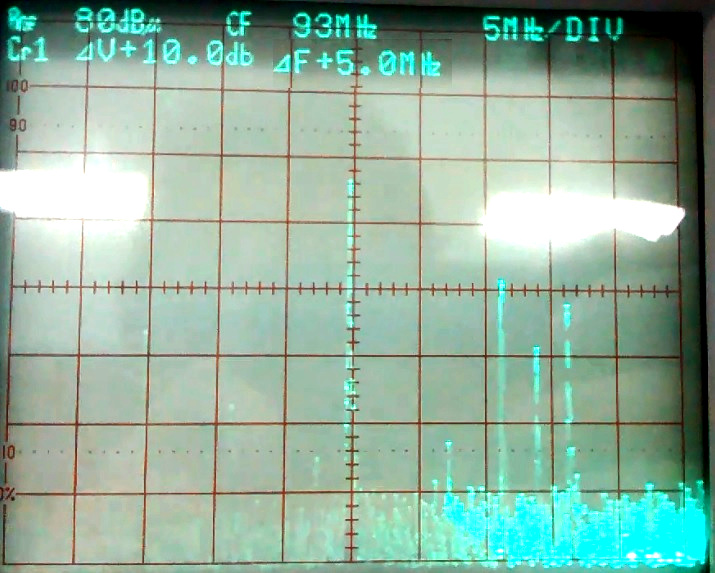
\includegraphics[scale=0.6]{imagem/analisador.jpg}
\caption{Analisador de espectro na frequência de transmissão}
\label{fig:analisador}
\end{figure}

Devido ao valor observado no analisador de espectro estar maior do que o valor esperado de $88MHz$, optou-se então por alterar o número de espiras do indutor para diminuir a frequência de transmissão.
Então com um indutor de 7 espiras foi possível enviar e receber o sinal senoidal de $1kHz$ na frequência de $88MHz$.

\newpage
\section{Conclusão}

Realizado a montagem do transmissor FM, foi possível validar as técnicas de projetos vistas em sala de aula. Mesmo os resultados obtidos sendo diferentes dos resultados esperados. Primeiramente, ao projetarmos, dada uma frequência da portadora de $88kHz$, o capacitor e o indutor, são necessários levar em conta a tolerância do capacitor, que é um componente comercial. Também devemos considerar o fato do circuito estar montado em uma protoboard, e isso somado ao fato de trabalharmos com um valor de capacitância muito baixo, as capacitâncias parasitas se tornam assim significantes. 

Dessa forma, para se aproximar da portadora desejada de $88kHz$, através de tentativas, foi aumentado o número de espiras até que um resultado satisfatório fosse alcançado, que no caso foi de 7 espiras, duas a mais do que o calculado.

\nocite{taufik}
\bibliographystyle{abbrv}
\bibliography{ref}

\end{document}
